\section{Technologien, Datenmodell und Umsetzung}
Dieses Kapitel erläutert zunächst die verwendeten Technologien, beschreibt anschliessend das definierte Datenmodell und zeigt abschliessend dessen Umsetzung in der entwickelten Lösung.

\subsection{Technologien}
Für die Realisierung des virtuellen Filesystems und die Entwicklung des Language Servers kommen Technologien zum Einsatz, welche sich eng an den bestehenden technischen Stack der Monidas-Plattform anlehnen. Die Wahl der eingesetzten Technologien erfolgte in Abstimmung mit dem Auftraggeber, um eine spätere Integration sowie Wartbarkeit und Erweiterbarkeit der entwickelten Lösung sicherzustellen. Nachfolgend werden die ausgewählten Technologien näher vorgestellt. 

%Zum Einsatz kommen dabei die Graphdatenbank Selva und das JavaScript-Framework Based, welche nachfolgend näher erläutert werden.

\subsubsection{Selva}
Dieses Unterkapitel beschreibt die im Projekt eingesetzte Graphdatenbank \textit{Selva}\footnote{\url{https://github.com/atelier-saulx/selva}}. Im Folgenden werden das zugrundeliegende Datenbankschema, die verwendete Query DSL sowie die API zur Interaktion mit der Datenbank vorgestellt.

%Selva wurde aufgrund ihrer Unterstützung für komplexe Graphstrukturen und Echtzeit-Abfragen ausgewählt, wodurch sie sich gut für die Anforderungen der Monidas-Plattform eignet.

\paragraph{Datenbankschema}
In Selva wird das Datenmodell über ein Schema definiert. Dieses Schema legt fest, welche Objekttypen existieren, über welche Felder diese verfügen und welche Datentypen dabei verwendet werden dürfen. Neben einfachen Datentypen wie \texttt{string}, \texttt{int} und \texttt{boolean} unterstützt Selva komplexe Beziehungstypen wie \texttt{reference} (für 0:1-Beziehungen) und \texttt{references} (für 0:n-Beziehungen).

Das Schema führt grundlegende Validierungen auf Datentypen-Ebene durch. Beispielsweise prüft Selva automatisch, ob Werte eines String-Feldes tatsächlich Zeichenketten sind oder ob Felder vom Typ email einem gültigen E-Mail-Format entsprechen.

Weitergehende Anforderungen wie Pflichtfelder (notNull), Pfadeinschränkungen (existsIn), bidirektionale Verknüpfungen (bidirectional) oder Erstellungseinschränkungen (canCreate) werden hingegen nicht automatisch unterstützt. Diese Anforderungen werden im Rahmen der Arbeit selbst definiert und validiert. Eine detaillierte Erläuterung dieser definierten Constraints erfolgt in Abschnitt \ref{sec:schema-umsetzung}.

%; deren konkrete Umsetzung in der Implementierung des virtuellen Filesystems wird dort ebenfalls beschrieben.
\pagebreak

Ein vereinfachtes Schema könnte wie folgt aussehen:

\lstdefinestyle{customtypescript}{
  belowcaptionskip=1\baselineskip,
  breaklines=true,
  frame=single,
  xleftmargin=\parindent,
  numbers=left,
  language=JavaScript,
  showstringspaces=false,
  basicstyle=\footnotesize\ttfamily\color{black},
  keywordstyle=\bfseries\color{black},
  commentstyle=\itshape\color{gray!60!black},
  identifierstyle=\color{black},
  stringstyle=\color{gray!20!black},
  numberstyle=\tiny\color{gray!50},
  rulecolor=\color{gray!70},
  backgroundcolor=\color{gray!10},
}

\lstinputlisting[
  caption={Beispiel für ein Selva-Datenbankschema}, 
  label={lst:schema_beispiel},
  style=customtypescript
]{listings/schema_bsp.json}


Im dargestellten Beispiel sind drei Objekttypen definiert: \texttt{Sensor}, \texttt{Location} und \texttt{Threshold}. Die Felder bilden sowohl einfache Attribute, beispielsweise Name und geografische Angaben, als auch Beziehungen zwischen den Objekten ab. Beispielsweise besitzt der \texttt{Sensor} eine eindeutige Standortzuweisung (\texttt{location}) und mehrere Grenzwerte (\texttt{thresholds}). 

%Die konkrete Verwendung und Umsetzung des Schemas wird in Abschnitt \ref{sec:schema-umsetzung} beschrieben.

\paragraph{Query Domain Specific Language (DSL)}
Um gezielt Daten abzufragen und zu bearbeiten, nutzt Selva eine eigene Query DSL. Diese DSL erlaubt die Definition von Abfragen über JavaScript-Objekte und legt gleichzeitig die Struktur der abgefragten Daten fest.

tbd alias 

%Selva ermöglicht es, Objekten zusätzlich zu ihrer ID einen lesbaren Alias zuzuweisen. Dies erleichtert den Zugriff, da Datenbankobjekte damit direkt über verständliche Namen angesprochen werden können. Die konkrete Nutzung und Verwaltung der Aliase in dieser Arbeit wird in Abschnitt XY genauer erläutert.

Dabei unterscheidet die Query DSL zwischen Feldern und Operatoren:

\begin{itemize} \item \textbf{Felder} repräsentieren gespeicherte Eigenschaften von Objekten. Mittels einer Query wird festgelegt, welche Eigenschaften im Ergebnis erscheinen sollen. Dabei können einfache Merkmale (wie Name oder Status eines Sensors) und auch komplexe, verknüpfte Informationen (etwa Standort oder Schwellenwerte) abgefragt werden.

\item \textbf{Operatoren} hingegen sind Anweisungen oder Befehle, die bestimmen, wie diese Daten im Ergebnis präsentiert werden (z. B. sortieren, filtern).
\end{itemize}

\paragraph{Selva-API}
Zur Interaktion zwischen Anwendung und Datenbank bietet Selva eine eigene API, welche grundlegende Operationen zur Datenmanipulation und -abfrage bereitstellt. Dazu gehören das Abfragen von Daten (\texttt{get}), das Erstellen und Aktualisieren von Objekten (\texttt{set}), das Löschen von Daten (\texttt{delete}) sowie das Beobachten von Datenänderungen in Echtzeit (\texttt{observe}). Weitere Funktionen der API ermöglichen das Abfragen (\texttt{getSchema}) und Anpassen (\texttt{updateSchema}) des Datenbankschemas, das Erzeugen eindeutiger IDs (\texttt{id}) sowie die Bestimmung des Objekttyps auf Basis einer ID (\texttt{getTypeFromId}).

Die praktische Verwendung aller genannten Operationen wird im Anhang \ref{sec:based-operationen} anhand konkreter Code-Beispiele gezeigt. Diese Operationen wurden für die Implementierung der im Rahmen dieser Arbeit entwickelten Funktionalitäten eingesetzt.

\subsubsection{Based}
Ergänzend zu Selva wird das JavaScript-Framework \textit{Based}\footnote{\url{https://github.com/atelier-saulx/based}} verwendet. Während Selva die direkte Speicherung und Abfrage der Daten verantwortet, bietet Based eine API zur Abstraktion und Vereinfachung der Kommunikation mit der Datenbank. Anwendungen interagieren ausschliesslich über Based, welches intern die benötigten Operationen auf Selva ausführt.

\begin{itemize} 
\item \textbf{Queries} dienen dem lesenden Zugriff auf gespeicherte Daten und ermöglichen sowohl einmalige Abfragen als auch sogenannte \textit{Subscriptions}. Mittels Subscriptions können Anwendungen auf Datenänderungen unmittelbar reagieren.

\item \textbf{Functions} hingegen führen schreibende Operationen aus, beispielsweise das Erstellen, Aktualisieren oder Löschen von Daten. Zusätzlich können Functions serverseitige Logik enthalten. Dadurch lassen sich Validierungen, Prüfungen oder komplexere Abläufe direkt auf dem Server umsetzen, bevor Daten gespeichert werden.
\end{itemize}



Die konkrete Verwendung der Queries und Functions sowie deren Zusammenspiel mit den zuvor beschriebenen Selva-Datenbankoperationen werden anhand exemplarischer Code-Beispiele im Anhang \ref{sec:selva-operationen} dargestellt.

\paragraph{VS Code}
VS Code dient als Plattform für zwei getrennte Extensions. Für das virtuelle Filesystem kommt die \textit{FileSystemProvider}-API\footnote{\url{https://code.visualstudio.com/api/references/vscode-api\#FileSystemProvider}} zum Einsatz. Die API stellt Funktionen bereit, um ein eigenes Filesystem mit Dateien und Ordnern über URI-Pfade zu verwalten. Dazu gehören das Erstellen, Löschen und Lesen von Inhalten. 

Für die Editorunterstützung wird das Language Server Protocol verwendet. Die Integration erfolgt nach den Vorgaben des offiziellen \textit{Language Server Extension Guide}\footnote{\url{https://code.visualstudio.com/api/language-extensions/language-server-extension-guide}}.

\textbf{tbd wird inhaltlich noch angepasst}

\paragraph{Node.js / TypeScript}
tbd

\pagebreak
\subsection{Architekturübersicht}
Nach der Vorstellung der verwendeten Technologien beschreibt dieser Abschnitt den Aufbau der Gesamtarchitektur. Für das Lesen der Arbeit stellt die Übersicht eine Orientierungshilfe dar, um die technische Gliederung der Lösung von Beginn an nachvollziehbar zu machen.

Die Lösung ist modular aufgebaut und besteht aus zwei getrennten Extensions. Eine ist für das virtuelle Filesystem zuständig, die andere für die Editorunterstützung. Der Editor ist die Schnittstelle, über die die Editorunterstützung auf die Inhalte des virtuellen Filesystem zugreift.

...tbd


\begin{figure}[H]
  \centering
  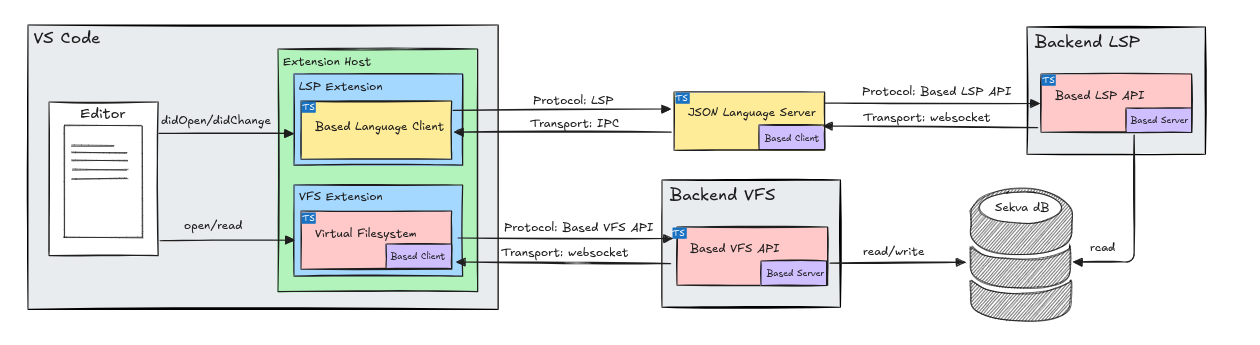
\includegraphics[width=\linewidth]{Arch.png}
  \caption{Architekturübersicht der implementierten Lösung}
  \label{fig:arch_modell}
\end{figure}

\subsection{Domänenmodell}
Im Rahmen der Arbeit kommt ein Domänenmodell aus dem Bereich E-Commerce zum Einsatz. Es dient als Beispiel und kann durch andere Modelle ersetzt werden, ohne dass die Funktionsweise der Lösung angepasst werden muss.


\subsubsection*{Constraints zur Steuerung des Anwendungsverhaltens}
Die Datenbank bietet keine nativen Mechanismen zur Durchsetzung von Modellregeln wie Kardinalitäten oder Referenzbeschränkungen. Um das Verhalten der Anwendung dennoch gezielt zu steuern, wurden im Schema drei Constraints definiert.

\begin{itemize}
 \item \textbf{notNull}: Markiert ein Feld als erforderlich.
  \item \textbf{existsIn}: Erlaubt nur Verweise auf Objekte eines bestimmten Typs, die an einem definierten Pfad gespeichert sind.
  \item \textbf{canCreate}: Erlaubt das Erstellen von untergeordneten Objekten.
  \item \textbf{bidirectional}: Erstellt automatisch eine Rückverknüpfung.
\end{itemize}

Standardmässig gelten folgende Regeln, wenn keine Constraints im Schema definiert werden: 

\begin{itemize}
  \item \textbf{notNull}: \texttt{false}
  \item \textbf{existsIn}: \texttt{all}
  \item \textbf{canCreate}: \texttt{true}
  \item \textbf{bidirectional}: \texttt{false}
\end{itemize}

Diese Regeln ermöglichen es, modelllogische Konzepte wie Komposition, Aggregation oder Assoziationen im Schemas zudefinieren.  

\subsubsection*{Entitäten im Modell}
Das Domänenmodell umfasst folgende Entitäten:

\paragraph{Customer}
Customer ist ein Kunde mit den Feldern \texttt{firstname}, \texttt{lastname}, \texttt{emailAddress} und \texttt{slug}.



\begin{figure}[H]
  \centering
  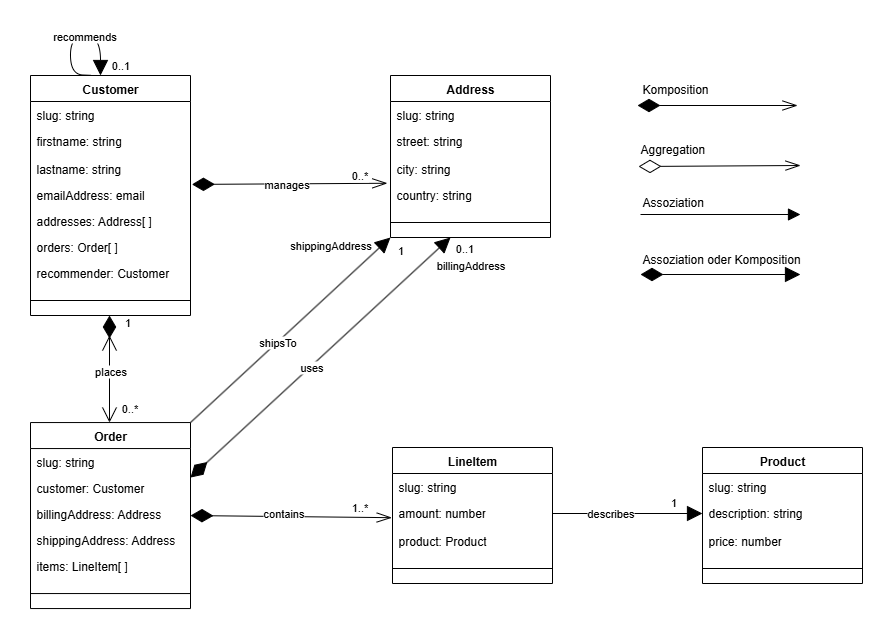
\includegraphics[width=\linewidth]{UML.png}
  \caption{UML-Modell mit Constraints zur Referenzierung und Erstellung}
  \label{fig:uml_modell}
\end{figure}


\subsection{Umsetzung als Datenbankschema}
\label{sec:schema-umsetzung}


\subsection{Analyse und Nutzung zur Laufzeit}
